%!TEX ROOT=../diploma-thesis.tex

\chapter{Anal\'yza}\label{ch:analyza}

Tato kapitola analyzuje problematiku byznysov\'ych pravidel v informačn\'{\i}ch systémech
a detailně popisuje architekturu orientovanou na služby, včetně jej\'{\i}ho historického
v\'yvoje a modern\'{\i}ho trendu v podobě microservices. Na základě toho kapitola popisuje nedostatky
současn\'ych př\'{\i}stupů při řešen\'{\i} průřezov\'ych problémů v těchto architekturách, s důrazem na byznysová pravidla.
V závěru kapitoly jsou identifikovány požadavky, které by měl splňovat framework,
jež bude v\'ystupem této diplomové práce.

\section{Byznysová pravidla}\label{sec:business-rules}

Informačn\'{\i} systémy (\gls{IS}) maj\'{\i} za úkol ulehčit, automatizovat či poskytovat podporu pro
byznysové procesy společnost\'{\i}, které je využ\'{\i}vaj\'{\i}. Tyto procesy jsou tedy stěžejn\'{\i}m
prvkem \gls{IS}. Systém má také za úkol uchovávat a spravovat data společnosti
a měl by zaručit, že nedojde k jejich poškozen\'{\i} či narušen\'{\i} jejich integrity.
Byznysové procesy, potažmo byznysové operace, proto musej\'{\i}
podléhat jasně definovan\'ym byznysov\'ym pravidlům, která zajišťuj\'{\i} konzistenci dat informačn\'{\i}ho
systému a také zabraňuj\'{\i} nepovolen\'ym operac\'{\i}m~\cite{cemus2015automated}.

Byznysová pravidla děl\'{\i}me do tř\'{\i} skupin~\cite{cemus2014aspect}:
\begin{description}
    \item [Bezkontextová pravidla] jsou validačn\'{\i} pravidla, která musej\'{\i} b\'yt obecně platná
    v každé operaci, jinak by mohlo doj\'{\i}t k porušen\'{\i} integrity dat systému. Př\'{\i}kladem může
    b\'yt pravidlo \uv{\textit{Adresa uživatele je platnou e-mailovou adresou}}.
    \item [Kontextová pravidla] jsou pravidla, která musej\'{\i} b\'yt zohledněna v daném kontextu
    byznysové operace, např\'{\i}klad \uv{\textit{Při přidán\'{\i} produktu do koš\'{\i}ku nesm\'{\i} součet položek
    v koš\'{\i}ku přesahovat částku milion korun}}
    \item [Průřezová pravidla] jsou parametrizována stavem systému nebo uživatelského účtu a maj\'{\i}
    dopad na velkou část byznysov\'ych operac\'{\i}. Uvažme pravidlo \uv{\textit{V systému nesm\'{\i} prob\'{\i}hat
    žádné změny po dobu účetn\'{\i} uzávěrky}}.
\end{description}

Dále také rozlišujeme dva typy byznysov\'ych pravidel, a těmi jsou \textit{preconditions}
a \textit{post-conditions}~\cite{cemus2015automated}.

\subsection{Precondition}

Aby mohla b\'yt byznysová operace vykonána, musej\'{\i}
b\'yt splněny předem definované podm\'{\i}nky, neboli předpoklady,
které naz\'yváme \textit{preconditions}. Pokud alespoň jedna z podm\'{\i}nek
nen\'{\i} splněna, byznysová operace nemůže proběhnout.

Pro lepš\'{\i} ilustraci uveďme př\'{\i}klad: aby mohla b\'yt provedena
registrace uživatele s danou emailovou adresu, mus\'{\i} b\'yt splněna
podm\'{\i}nka, že uživatel vyplnil svoj\'{\i} emailovou adresu, a zároveň
dosud v systému neexistuje žádn\'y uživatel se stejnou emailovou adresou.

\subsection{Post-condition}

Na byznysovou operaci mohou b\'yt kladeny požadavky, které
musej\'{\i} b\'yt splněny po jej\'{\i}m úspěšném vykonán\'{\i}. Př\'{\i}kladem
může b\'yt anonymizace uživatelů při vytvářen\'{\i} statistického
reportu e-commerce společnosti – po vygenerován\'{\i} reportu
post-condition zajist\'{\i}, že z něj budou smazány veškeré citlivé údaje.
Dalš\'{\i}m př\'{\i}padem může b\'yt filtrován\'{\i} v\'ystupu byznysové operace.
Např\'{\i}klad při v\'ypisu objednávek pro zákazn\'{\i}ka se chceme ujistit, že
všechny vypsané objednávky patř\'{\i} danému zákazn\'{\i}kovi.

\subsection{Reprezentace byznysového pravidla}

Existuje několik možnost\'{\i}, jak zachytit a reprezentovat byznysová pravidla~\cite{cemus2015automated}.
Nejběžnějš\'{\i} a nejpouž\'{\i}vanějš\'{\i} metodou je jejich zachycen\'{\i} v programovac\'{\i}m
jazyce. Tato metoda je snadná, protože programátor může použ\'{\i}t stejn\'y jazyk
pro popis pravidel stejně jako pro popis celého systému. Bohužel, tato metoda
nám nedává př\'{\i}liš možnost\'{\i} jak provést inspekci a extrakci pravidel.
Dalš\'{\i}, pokročilejš\'{\i} metodou, je zápis pravidel pomoc\'{\i} meta-instrukc\'{\i}, např\'{\i}klad anotac\'{\i},
nebo tzv.\textit{Expression Language} (\gls{EL}). Tato metoda poskytuje dobrou možnost inspekce,
ale zpravidla nen\'{\i} typově bezpečná a může snáze způsobovat chyby v programu.
Posledn\'{\i}, nejpokročilejš\'{\i} metodou, je zápis pomoc\'{\i} doménově specifick\'ych jazyků.
Ty jsou snadno srozumitelné nejen pro programátory, ale i pro doménové experty.
Nevyžaduj\'{\i} inspekci a mohou b\'yt typově bezpečné. Mezi jejich nev\'yhody ale patř\'{\i} vysoká
počátečn\'{\i} investice v podobě návrhu takového jazyka a nutnost jeho kompilace nebo
interpretace.

\subsection{Byznysov\'y kontext}

Informačn\'{\i} systém zpravidla implementuje v\'{\i}ce byznysov\'ych procesů, které se vážou
na jeden či v\'{\i}ce uživatelsk\'ych scénářů. Uživatelsk\'y scénář se pak děl\'{\i} na jednotlivé
kroky, např\'{\i}klad zaslán\'{\i} potvrzovac\'{\i}ho e-mailu k objednávce, či uložen\'{\i} objednávky
do databáze. Tyto kroky naz\'yváme \textit{byznysové operace} – tedy operace, které maj\'{\i}
byznysovou hodnotu. Ke každé byznysové operaci př\'{\i}sluš\'{\i} množina byznysov\'ych pravidel,
konkrétně preconditions a post-conditions.

Při běhu informačn\'{\i}ho systému je v paměti držen tzv. \textit{exekučn\'{\i} kontext} (z anglického \textit{execution context}),
kter\'y se skládá z několika d\'{\i}lč\'{\i}ch kontextů~\cite{cemus2017separation}. Prvn\'{\i}m
je \textit{aplikačn\'{\i} kontext} (z anglického \textit{application context}), ve kterém je uložen stav globálnc\'{\i}h proměnn\'ych systému,
jako např. nastaven\'{\i} produkčn\'{\i}ho režimu, nebo př\'{\i}znak o tom, zda právě prob\'{\i}há obchodn\'{\i}
uzávěrka. Dalš\'{\i}m je \textit{uživatelsk\'y kontext}, kter\'y obsahuje informace o aktuálně
přihlášeném uživateli. \textit{Kontext požadavku} (z anglického \textit{Request context}) obsahuje
informace o aktuáln\'{\i}m požadavku, jako IP adresa uživatele či jeho geolokace,
a vztahuje se zejména k webov\'ym službám. Posledn\'{\i}m je \textit{byznysov\'y kontext}. Ten
chápeme jako množinu preconditions a post-conditions s byznysovou hodnotou, která se
váže na konkrétn\'{\i} byzynsovou operaci~\cite{cemus2015automated}.
Abychom mohli efektivně definovat co nejširš\'{\i} škálu byzynsov\'ych pravidel,
musej\'{\i} při jejich vyhodnocován\'{\i} b\'yt dostupné proměnné exekučn\'{\i}ho kontextu,

\section{Architektura orientovaná na služby}\label{sec:soa}

\textit{Architektura orientovaná na služby} (\gls{SOA}) je odpovědí na stále se zvyšující
nároky na informační systémy a jejich rostoucí velikost. Na rozd\'{\i}l od \textit{monolitické architektury},
děl\'{\i} \gls{SOA} systém na samostatné nezávislé celky, zvané \textit{služby}, které jsou
poskytují d\'{\i}lč\'{\i} části požadované funkcionality systému.
Historicky byl term\'{\i}n \gls{SOA} vykládán několika způsoby a představoval
několik rozd\'{\i}ln\'ych, nekompatibiln\'{\i}ch konceptů~\cite{fowler2005serviceorientedambiguity}.
Absence kvalitn\'{\i}ch definic služby a obecně \gls{SOA} vedla k v posledn\'{\i} době i ke snahám
o opuštěn\'{\i} tohoto konceptu~\cite{cerny2017disambiguation}.
Pro lepší porozumění se tato kapitola věnuje stručnému historickému přehledu \gls{SOA}
a shrnuje výhody a nevýhody jednotlivých přístupů.

\subsection{Common Object Request Broker Architecture}\label{sec:corba}

Prvn\'{\i}m historick\'ym předchůdcem architektury orientované na služby
byla tzv. \textit{Common Object Request Broker Architecture}
(\gls{CORBA})~\cite{siegel2000corba}. Ta umožňuje vzájemnou komunikaci aplikací
implementovan\'ych v různ\'ych technologi\'{\i}ch. Její základní komponentou je
je \textit{Object Request Broker} (\gls{ORB}), kter\'y emuluje objekty,
na kter\'ych může klient volat jejich metody. Při zavolán\'{\i} metody
na objektu, kter\'y se fyzicky nacház\'{\i} na vzdáleném stroji,
zprostředkovává \gls{ORB} veškerou komunikaci a poskytuje kompletn\'{\i} rozhran\'{\i}
volaného objektu. Komunikace se vzdálen\'ym objektem s sebou však nese celou řadu problémů,
např\'{\i}klad vyšš\'{\i} latenci při komunikaci nebo v\'yjimečné stavy, které je potřeba
ošetřit, či obížnou optimalizaci kódu využívající \gls{ORB}.

\subsection{Web Services}

Nedostatky architektury \gls{CORBA} vedly k vývoji jednodušš\'{\i}ho
a kvalitnějšího formátu pro popis komunikace služeb. Volán\'{\i} metod na vzdálen\'ych objektech
bylo nahrazeno explicitn\'{\i}m pos\'{\i}lán\'{\i}m zpráv mezi službami pomocí protokolu \gls{HTTP}.
Pro popis schématu zpráv vznikl formát \textit{Simple Object Access
Protocol} (\gls{SOAP})~\cite{box2000simple}, kter\'y v kombinaci s
\textit{Web Service Description Language} (\gls{WSDL})~\cite{christensen2001web}
umožňuje kompletn\'{\i} definici rozhran\'{\i} pro komunikaci mezi službami.

\subsection{Message Queue}

\begin{figure}
    \centering
    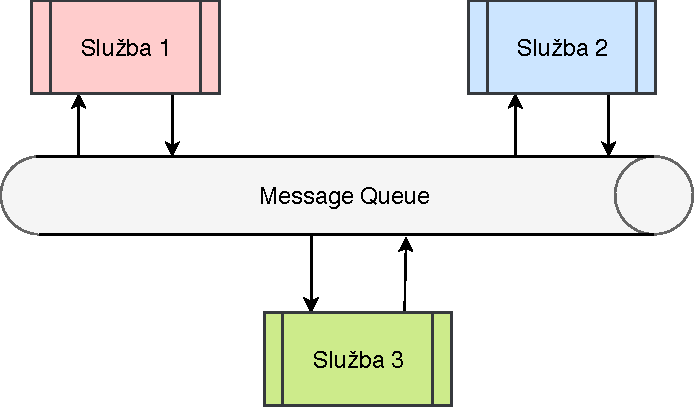
\includegraphics[keepaspectratio=true, width=0.5\linewidth]{figures/message-queue.pdf}
    \caption{Komunikace služeb pomoc\'{\i} Message Queue}
    \label{fig:message-queue}
\end{figure}

Dalš\'{\i}m z konceptů, kter\'y v rámci \gls{SOA} vznikl, je tzv. \textit{Message Queue} (\gls{MQ}).
Základn\'{\i} myšlenkou \gls{MQ}, znázorněnou na obrázku~\ref{fig:message-queue},
je asynchronn\'{\i} komunikace služeb pomoc\'{\i} zpráv nezávisl\'ych
na platformě. Komunikaci zprostředkovává fronta, která přij\'{\i}má a rozes\'{\i}lá
zprávy mezi službami. To přináš\'{\i} vyšš\'{\i} škálovatelnost a menš\'{\i} provázanost
mezi službami. Všechny služby ale mus\'{\i} použ\'{\i}vat jednotn\'y formát zpráv.

\subsection{Enterprise Service Bus}

Ačkoliv zm\'{\i}něné modely usnadňuj\'{\i} komunikaci služeb a zvyšuj\'{\i} jejich
spolehlivost, integrace služeb může b\'yt obt\'{\i}žná, pokud služby použ\'{\i}vaj\'{\i}
navzájem různé komunikačn\'{\i} protokoly a formáty. Tento problém řeší \textit{Enterprise Service
Bus} (\gls{ESB})~\cite{chappell2004enterprise}, znázorněn\'y na obrázku~\ref{fig:enterprise-service-bus},
kter\'y má za úkol propojit heterogenn\'{\i} služby a sestavit mezi nimi komunikačn\'{\i} kanály.
T\'{\i}m na sebe \gls{ESB} přeb\'{\i}rá zodpovědnost za překlad jednotliv\'ych zpráv a centralizuje
veškerou komunikaci v systému.

\begin{figure}
    \centering
    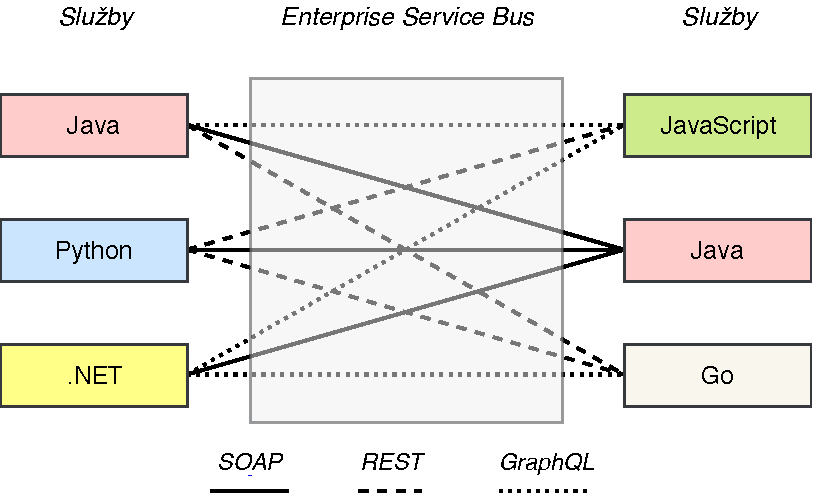
\includegraphics[keepaspectratio=true, width=0.7\linewidth]{figures/enterprise-service-bus.pdf}
    \caption{Komunikace služeb skrz Enterprise Service Bus}
    \label{fig:enterprise-service-bus}
\end{figure}

\subsection{Microservices}\label{sec:microservices}

%\goal{Microservices a budoucnost SOA}
Moderní architektura \textit{Microservices} přináš\'{\i} soubor konceptů, které specializuj\'{\i} a konkretizuj\'{\i}
principy \gls{SOA}. Microservices se tedy dá chápat jako podmnožina \gls{SOA}, ačkoliv existují i názory,
že jde o odlišné architektury~\cite{richards2015microservices}. Základn\'{\i} myšlenkou je v\'yvoj informačn\'{\i}ho
systému jako množiny mal\'ych oddělen\'ych služeb, které jsou spouštěny v samostatn\'ych procesech
a komunikuj\'{\i} spolu pomoc\'{\i} jednoduch\'ych protokolů~\cite{lewis2014microservices}.
Microservices preferují decentralizaci a samostatnost služeb.

%\goal{Stavba služeb kolem byznysov\'ych schopnost\'{\i}}
Microservices se zaměřují na organizaci služeb kolem byznysov\'ych schopnost\'{\i} systému.
Nam\'{\i}sto horizontáln\'{\i}ho dělen\'{\i} systému podle jeho vrstev\footnote{
Zde předpokládáme klasickou tř\'{\i}vrstvou architekturu~\cite{fowler2002patterns},
rozděluj\'{\i}c\'{\i} systém na \textit{datovou vrstvu}, \textit{aplikačn\'{\i} vrstvu}
a \textit{prezentačn\'{\i} vrstvu}. Tyto vrstvy maj\'{\i} oddělené zodpovědnosti a komunikuj\'{\i}
spolu pomoc\'{\i} jasně definovan\'ych společn\'ych rozhran\'{\i}.
} navrhuje rozdělit systém vertikálně podle jeho byznysov\'ych schopnost\'{\i}.
Na obrázku~\ref{fig:monolith-vs-microservices} je toto rozdělen\'{\i} demonstrováno.

\begin{figure}
    \centering
    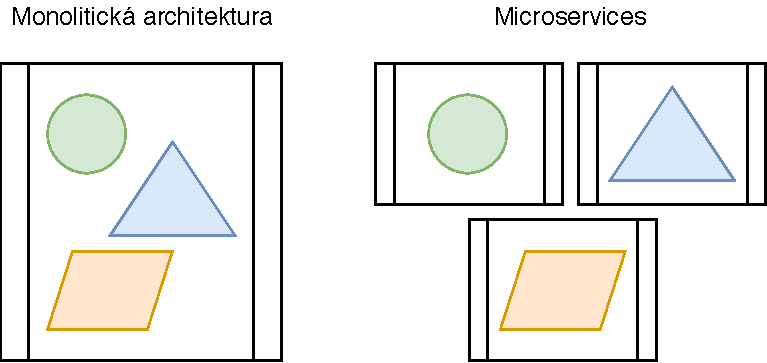
\includegraphics[keepaspectratio=true, width=0.5\linewidth]{figures/monolith-vs-microservices.pdf}
    \caption{Porovnán\'{\i} struktury monolitické architektury a microservices~\cite{lewis2014microservices}}
    \label{fig:monolith-vs-microservices}
\end{figure}

%\goal{Myšlenka nahraditelnosti komponenty}
%Koncept microservices přem\'yšl\'{\i} o službě jako o samostatné komponentě,
%kterou lze individuálně vyměnit či vylepšit, bez nutnosti zásahu do
%ostatn\'{\i}ch služeb~\cite{lewis2014microservices}. Monolitická architektura
%vyžaduje i při malé změně jedné části cel\'y systém znovu zkompilovat, sestavit
%a nasadit. Malé služby slouž\'{\i}c\'{\i} ideálně jedinému byznysovému účelu lze naopak
%při změně byznysov\'ych požadavků snadno nahradit samostatně bez zásahu do zbytku
%systému. T\'{\i}m se usnadňuje cyklus nasazen\'{\i} a spuštěn\'{\i} nové verze služby.

%\goal{Myšlenka smart endpoints, dumb pipes}
%Microservices také přinášej\'{\i} koncept \uv{smart endpoint, dumb pipes},
%kter\'y opoušt\'{\i} koncept \gls{ESB} ve prospěch přesunut\'{\i} veškeré byznysové logiky
%na stranu služeb. T\'{\i}m se zvyšuje zapouzdřenost služeb a snižuje se
%jejich vzájemné provázán\'{\i}. Nutno podotknout, že microservices často
%využ\'{\i}vaj\'{\i} ke své funkci Message Queues.

%\paragraph{Škálovatelnost}
%Dalš\'{\i} nespornou v\'yhodou microservices je vysoká škálovatelnost systému. Pokud je na
%některou ze služeb kladen vyšš\'{\i} nárok na v\'ykon než na ostatn\'{\i}, maj\'{\i}
%v\'yvojáři možnost konkrétn\'{\i} službu horizontálně škálovat aniž by
%museli škálovat kompletně cel\'y systém, na rozd\'{\i}l od monolitické architektury.
%Srovnán\'{\i} př\'{\i}stupů je znázorněno na obrázku~\ref{fig:microservices-deployment}.
%D\'{\i}ky této vlastnosti je možné sn\'{\i}žit nároky na systémové zdroje při zachován\'{\i}
%stejného v\'ykonu.

%\paragraph{Využit\'{\i} rozlišn\'ych technologi\'{\i}}
%Monolitické aplikace jsou často implementovány v jednom programovac\'{\i}m jazyce
%a využ\'{\i}vaj\'{\i} omezenou množinu technologi\'{\i}. Ne pro každ\'y úkol je ale vhodn\'y
%jeden programovac\'{\i} jazyk a s rostouc\'{\i} velikost\'{\i} informačn\'{\i}ho systému často roste
%i rozmanitost jeho funkcionality. Rozdělen\'{\i}m systému na v\'{\i}ce služeb, které
%komunikuj\'{\i} protokolem nezávisl\'ym na platformě, je v\'yvojářům umožněno využ\'{\i}t
%širš\'{\i} spektrum technologi\'{\i} a implementovat požadovanou funkcionalitu
%efektivněji.

%\begin{figure}
%    \centering
%    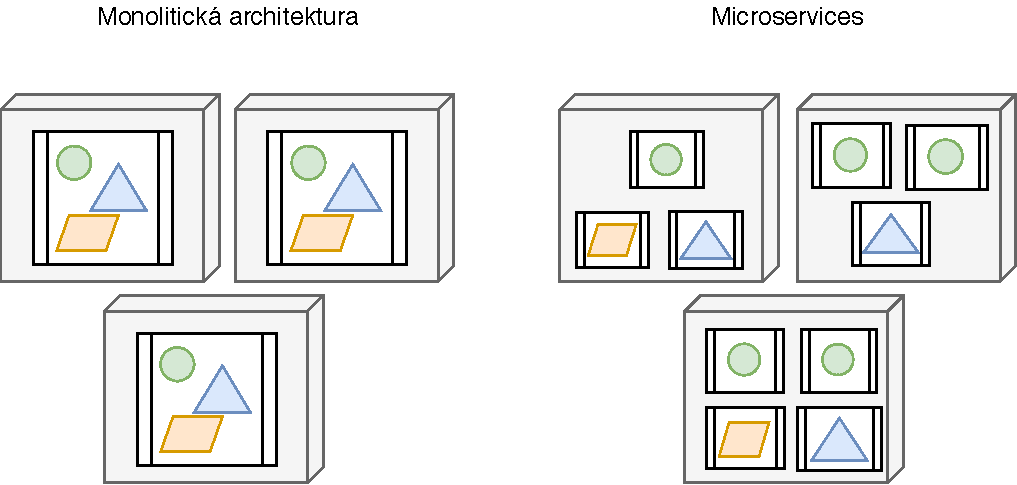
\includegraphics[keepaspectratio=true, width=0.8\linewidth]{figures/microservices-deployment.pdf}
%    \caption{Porovnán\'{\i} nasazen\'{\i} monolitické architektury a microservices~\cite{lewis2014microservices}}
%    \label{fig:microservices-deployment}
%\end{figure}

%\paragraph{Decentralizace úložiště}
%Dalš\'{\i}m z principů, které microservices přináš\'{\i}, je oddělen\'{\i} a decentralizace
%databázového úložiště. Každá služba, či cluster instanc\'{\i} jedné služby, zapisuj\'{\i}
%a čtou data ze své oddělené databáze. Pokud potřebujou nač\'{\i}st data jiné služby,
%musej\'{\i} k tomu využ\'{\i}t jej\'{\i} \gls{API}. T\'{\i}m se ještě v\'yrazněji odděluje zodpovědnost služeb.
%Typickou praktikou v rámci \gls{SOA} je naopak sd\'{\i}len\'{\i} jedné databáze mezi v\'{\i}ce službami,
%což je často dáno komerčn\'{\i}m modelem extern\'{\i}ho dodatavele databáze. Jediná databáze
%má nav\'{\i}c obrovskou v\'yhodu v transakčn\'{\i}m zpracován\'{\i}, které je centralizované.
%V př\'{\i}padě microservices je nutno transakce řešit distribuovaně, což je velmi náročn\'y
%úkol a společnosti často vol\'{\i} koncept tzv. \textit{eventual consistency}, kdy je
%preferována občasná nekonzistence v datech, která je následně manuálně opravena.
%Tento př\'{\i}stup je opodstatněn t\'{\i}m, že občasná manuáln\'{\i} oprava může b\'yt
%často levnějš\'{\i} než investice do kvalitn\'{\i}ho řešen\'{\i} distribuovan\'ych transakc\'{\i} –
%zejména pokud by jeho řešen\'{\i} znamenalo zpožděn\'{\i} v\'yvoje produktu a způsobilo
%by ztrátu obchodn\'{\i} př\'{\i}ležitosti~\cite{lewis2014microservices}.

\subsection{Orchestrace a choreografie služeb}

Základní podmínkou pro správnou funkci systému stavějícímu na \gls{SOA} je správná
komunikace a spolupráce jednotlivých služeb. K tomu slouží dva odlišné přístupy \textendash\xspace
\textit{orchestrace služeb} a \textit{choreografie služeb}.

\paragraph{Orchestrace služeb}
\textit{Orchestrace služeb} má za úkol zajistit, že komunikace mezi službami
proběhne úspěšně a ve správném časovém sledu~\cite{orchestration},
za použití centráln\'{\i} komponenty \textendash\xspace tzv. \textit{dirigenta}.
Typicky je jako dirigent využ\'{\i}ván \gls{ESB}, kter\'y je pro tuto roli vhodn\'y,
protože má informace o lokaci jednotliv\'ych služeb a zprostředkovává mezi nimi
komunikačn\'{\i} kanály.

\paragraph{Choreografie služeb}
Př\'{\i}m\'ym opakem orchestrace je tzv. \textit{choreografie služeb} a znamená
vykonáván\'{\i} byznysov\'ych operac\'{\i} autonomně a asynchronně, bez centráln\'{\i}
autority. Tento př\'{\i}stup je preferován zejména v rámci microservices~\cite{dragoni2017microservices},
protože orchestrace vede k vyšš\'{\i}mu provázán\'{\i} služeb a nerovnoměrnému rozložen\'{\i}
zodpovědnost\'{\i} v systémů. Porovnán\'{\i} obou př\'{\i}stupů je graficky
znázorněno na obrázku~\ref{fig:choreography-orchestration}.

\begin{figure}
    \centering
    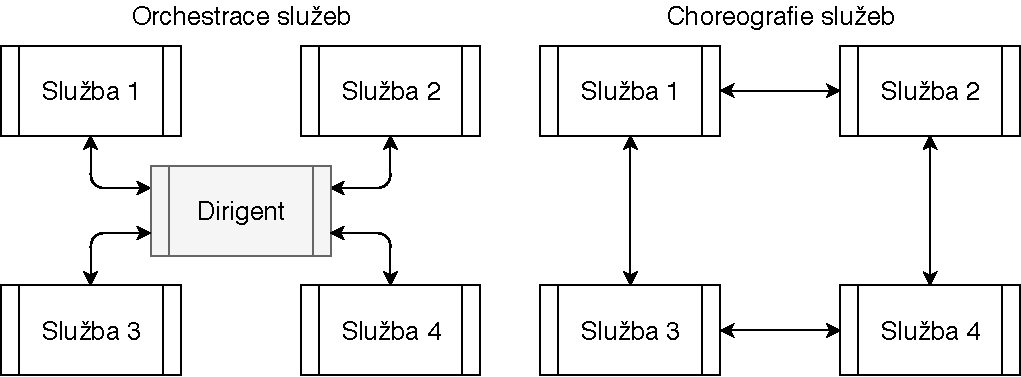
\includegraphics[keepaspectratio=true, width=0.8\linewidth]{figures/choreography-orchestration.pdf}
    \caption{Porovnán\'{\i} orchestrace a choreografie služeb~\cite{cerny2017disambiguation}}
    \label{fig:choreography-orchestration}
\end{figure}

% TODO: napsat o AI pro choreografii
~\cite{rao2004survey}

\subsection{Shrnutí}

Z předchozího textu lze vyvodit, že \gls{SOA}

\section{Nedostatky současného př\'{\i}stupu}\label{sec:shortcomings}

%\goal{Navázán\'{\i} na předchoz\'{\i} sekci}
%% TODO: toto přepsat nebo zahodit
%\gls{SOA} se zaměřuje zejména na dělen\'{\i} systému na služby a detailně rozeb\'{\i}rá
%formu jejich vzájemné komunikace. Neodpov\'{\i}dá ale na několik závažn\'ych otázek, se kter\'ymi se v praxi musej\'{\i}
%architekti informačn\'{\i}ch systémů vypořádat, aby architektura byla schopná uspokojivě
%plnit požadavky, které jsou na n\'{\i} kladené.

\goal{Problémy SOA a průřezov\'ych problémů}
Jelikož jedn\'{\i}m z c\'{\i}lů \gls{SOA}, potažmo microservices, je co nejv\'{\i}ce izolovat
jednotlivé služby, maj\'{\i} tyto architektury tendenci duplikovat části kódu
zajišťuj\'{\i}c\'{\i} funkcionalitu, která vyžaduje konzistentn\'{\i} zpracován\'{\i} ve v\'{\i}ce
službách~\cite{cerny2017disambiguation}, tzv. \textit{průřezov\'ych
problémů} (z anglického \textit{cross-cutting concerns}).
Př\'{\i}kladem mohou b\'yt právě byznysová pravidla~\cite{cemus2014aspect}, která je potřeba
zohlednit v rámci různ\'ych byznysov\'ych kontextů realizovan\'ych ve v\'{\i}ce službách.
Mezi dalš\'{\i} př\'{\i}klady se řad\'{\i} logován\'{\i}, monitoring či sběr dat
o telemetrii procesů.

\goal{Nast\'{\i}něn\'{\i} konkrétn\'{\i}ho př\'{\i}kladu}
Pro lepší představu diskutovaného problému uvažme e-commerce systém
skládaj\'{\i}c\'{\i} se z několika služeb naprogramovan\'ych v různ\'ych technologi\'{\i}ch,
a procesy vytváření faktury a vytváření objednávky, každý z nich implementovaný jinou službou.
Systém navíc obsahuje službu poskytující webové uživatelské rozhraní.
Při vytvářen\'{\i} faktury za objednávku mus\'{\i} b\'yt nejprve zvalidována fakturačn\'{\i} adresa.
Protože by mohla nastat situace, kdy by v př\'{\i}padě nevalidn\'{\i} adresy museli zaměstnanci
společnosti kontaktovat zákazn\'{\i}ka \textendash\xspace pokud vůbec takovou možnost maj\'{\i}
\textendash\xspace musí být adresa validována již při vytvářen\'{\i} objednávky.
V ideáln\'{\i}m př\'{\i}padě by navíc měl zákazn\'{\i}k být upozorněn na nevalidn\'{\i} fakturačn\'{\i}
adresu co nejdříve, ještě před odeslán\'{\i}m objednávkového formuláře př\'{\i}mo v uživatelském
rozhran\'{\i}~\cite{cemus2017separation}. Pro lepš\'{\i} představu je problém znázorněn na
obrázku~\ref{fig:service-cutting},

\goal{Náročná údržba a reakce na změnu požadavku}
Na příkladu lze pozorovat, že stejná funkcionalita se prom\'{\i}tá
do tř\'{\i} služeb, z nichž každá má zodpovědnost za jiné byznysové operace.
Stejn\'y kód, kter\'y realizuje validaci fakturačn\'{\i} adresy,
mus\'{\i} b\'yt implementován v každé ze zmiňovaných služeb,
v tomto př\'{\i}padě nav\'{\i}c ve třech různ\'ych programovac\'{\i}ch jazyc\'{\i}ch.
Pokud by vzešel změnový požadavek na validaci fakturačn\'{\i} adresy, změnu by bylo nutno
provést konzistentně na třech různ\'ych m\'{\i}stech, všechny tři služby znovu
sestavit a nasadit ve správném pořad\'{\i} tak, aby nedošlo k nekonzistení validaci adresy
při provádění jednotlivých byznysových operací.
\changed{Změny byznysových pravidel se dějí častěji, než změny kódu a struktury samotných
služeb v \gls{SOA}~\cite{rosenberg2005business}. Pokud je potřeba s každou změnou
byznysového pravidla sestavit a nasadit minimálně jednu službu, dramaticky
se zvyšuje náročnost na údržbu takového systému.
}

\goal{Microservices neř\'{\i}ká nic o tom, jak velké je mikro}
Problém validace fakturačn\'{\i}ch adres by bylo možné vyřešit vyčleněn\'{\i}m této funkcionality
do samostatné služby a vystavit jej\'{\i} rozhran\'{\i} pro ostatn\'{\i} služby,
Pokud však služby nesou př\'{\i}liš málo odpovědnosti,
nasazen\'{\i} a provoz každé služby s sebou přináš\'{\i} náklady nav\'{\i}c.
S rostouc\'{\i}m počtem průřezov\'ych problémů by tak rychle rostl
i počet služeb v systému a celkové náklady na jeho v\'yvoj a údržbu.

\begin{figure}
    \centering
    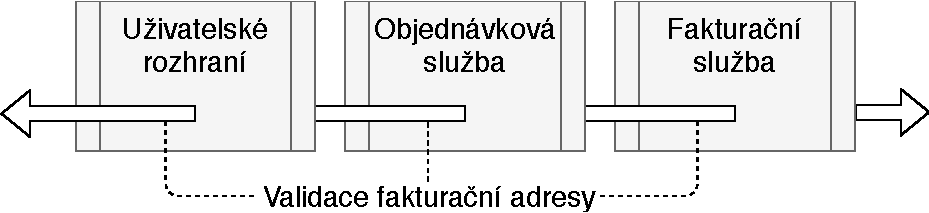
\includegraphics[keepaspectratio=true, width=0.8\linewidth]{figures/service-cutting.pdf}
    \caption{Př\'{\i}klad zásahu jedné funkcionality do v\'{\i}ce služeb}
    \label{fig:service-cutting}
\end{figure}

\section{Identifikace požadavků na implementaci frameworku}\label{sec:implementation-requirements}

Z př\'{\i}kladu popsaného v\'yše lze identifikovat požadavky, které by měly
b\'yt zohledněny při návrhu a implementaci frameworku pro centráln\'{\i} administraci
a automatickou distribuci byznysov\'ych pravidel v architektuře orientované na služby.

Framework, resp. jeho knihovny, by měly umožňovat:

\begin{itemize}
    \item{Definice byznys kontextů pomoc\'{\i} platformně nezávislého doménově specifického jazyka srozumitelného pro doménové experty}
    \item{Zápis preconditions a post-conditions pravidla jednotliv\'ych byznys kontextů}
    \item{Možnost jednoho kontextu rozšiřovat jiné kontexty}
    \item{Možnost centrálně spravovat byznysové kontexty, včetně úpravy stávaj\'{\i}c\'{\i}ch a vytvářen\'{\i} nov\'ych kontextů, to vše dynamicky za běhu systému}
    \item{Automatickou distribuci kontextů, vyhodnocován\'{\i} jejich preconditions a aplikaci post-conditions}
    \item{Možnost využ\'{\i}vat framework na v\'{\i}ce plaformách}
\end{itemize}

\section{Shrnut\'{\i}}

Tato kapitola analyzovala koncept byznysov\'ych pravidel a byznysov\'ych kontextů. Dále se věnovala architektuře orientované na služby,
jej\'{\i}m podobám, v\'yhodám a nev\'yhodám, a identifikovala nedostatky současn\'ych př\'{\i}stupů v řešen\'{\i} průřezov\'ych problémů,
které zasahuj\'{\i} do v\'{\i}ce služeb najednou. Nakonec byly identifikovány požadavky, které by měl splňovat framework, jež bude
v\'ystupem této práce.
